\documentclass[a4paper,11pt,]{book} % draft

\usepackage{silence}
\WarningFilter{fourier}{Please consider}
\WarningFilter{hyperref}{Token not allowed in a PDF string}

\usepackage[T1]{fontenc}
\usepackage{fontspec}
\usepackage[french,english]{babel}
\setmonofont{Ubuntu Mono}
\setlength{\textwidth}{146.8mm}
\setlength{\oddsidemargin}{11.6mm}
\setlength{\evensidemargin}{0.8mm}
\setlength{\topmargin}{-2.2mm}
\setlength{\textheight}{221.9mm}
\setlength{\headheight}{14pt}

\usepackage{setspace}
\setstretch{1.1}
\makeatletter
\setlength{\@fptop}{0pt}
\makeatother

\usepackage{lmodern}
\usepackage{fourier}
\usepackage{graphicx}
\usepackage{xcolor}
\usepackage{booktabs}
\usepackage{lipsum}
\usepackage[final]{microtype}
\usepackage[hyphens]{url}

\usepackage{fancyhdr}
\renewcommand{\sectionmark}[1]{\markright{\thesection\ #1}}
\pagestyle{fancy}
  \fancyhf{}
  \renewcommand{\headrulewidth}{0.4pt}
  \renewcommand{\footrulewidth}{0pt}
  \fancyhead[OR]{\bfseries \nouppercase{\rightmark}}
  \fancyhead[EL]{\bfseries \nouppercase{\leftmark}}
  \fancyfoot[EL,OR]{\thepage}
\fancypagestyle{plain}{
  \fancyhf{}
  \renewcommand{\headrulewidth}{0pt}
  \renewcommand{\footrulewidth}{0pt}
  \fancyfoot[EL,OR]{\thepage}}
\fancypagestyle{addpagenumbersforpdfimports}{
  \fancyhead{}
  \renewcommand{\headrulewidth}{0pt}
  \fancyfoot{}
  \fancyfoot[RO,LE]{\thepage}
}

\usepackage[final]{hyperref}
\definecolor[named]{purplish}{cmyk}{0.55,1,0,0.15}
\definecolor[named]{darkblueish}{cmyk}{1,0.58,0,0.21}
\hypersetup{
  colorlinks=true,
  pdfborder={0 0 0},
  linkcolor=purplish,
  citecolor=purplish,
  urlcolor=darkblueish,
  filecolor=darkblueish}
\urlstyle{same}
\usepackage[final]{pdfpages}
\usepackage{bookmark}

\makeatletter
\renewcommand\@pnumwidth{20pt}
\makeatother

\makeatletter
\def\cleardoublepage{\clearpage\if@twoside \ifodd\c@page\else
    \hbox{}
    \thispagestyle{empty}
    \newpage
    \if@twocolumn\hbox{}\newpage\fi\fi\fi}
\makeatother \clearpage{\pagestyle{plain}\cleardoublepage}

\usepackage{color}
\usepackage{tikz}
\usepackage[explicit]{titlesec}
\newcommand*\chapterlabel{}
\titleformat{\chapter}[display]
  {\normalfont\bfseries\Huge}
  {\gdef\chapterlabel{\thechapter\ }}
  {0pt}
    {\begin{tikzpicture}[remember picture,overlay]
    \node[yshift=-8cm] at (current page.north west)
      {\begin{tikzpicture}[remember picture, overlay]
        \draw[fill=black] (0,0) rectangle(35.5mm,15mm);
        \node[anchor=north east,yshift=-7.2cm,xshift=34mm,minimum height=30mm,inner sep=0mm] at (current page.north west)
        {\parbox[top][30mm][t]{15mm}{\raggedleft \rule{0cm}{0.6cm}\color{white}\chapterlabel}};  %the empty rule is just to get better base-line alignment
        \node[anchor=north west,yshift=-7.2cm,xshift=37mm,text width=\textwidth,minimum height=30mm,inner sep=0mm] at (current page.north west)
              {\parbox[top][30mm][t]{\textwidth}{\rule{0cm}{0.6cm}\color{black}#1}};
       \end{tikzpicture}
      };
   \end{tikzpicture}
   \gdef\chapterlabel{}
  } % code before the title body
\titlespacing*{name=\chapter,numberless}{-3.7cm}{83.2pt-\parskip}{\parskip+\parskip}
\titlespacing*{\chapter}{-3.7cm}{50pt-\parskip-\parskip}{\parskip+\parskip}
\titlespacing*{\section}{0pt}{13.2pt}{1em-\parskip}  % 13.2pt is line spacing for a text with 11pt font size
\titlespacing*{\subsection}{0pt}{13.2pt}{1em-\parskip}
\titlespacing*{\subsubsection}{0pt}{13.2pt}{1em-\parskip}
\titlespacing*{\paragraph}{0pt}{13.2pt}{1em-\parskip}

\newcounter{myparts}
\newcommand*\partlabel{}
\titleformat{\part}[display]  % type (section,chapter,etc...) to vary,  shape (eg display-type)
  {\normalfont\bfseries\Huge} % format of the part
  {\gdef\partlabel{\thepart\ }}     % the label
  {0pt} % separation between label and part-title
    {\ifpdf\setlength{\unitlength}{20mm}\else\setlength{\unitlength}{0mm}\fi
    \addtocounter{myparts}{1}
    \begin{tikzpicture}[remember picture,overlay]
    \node[anchor=north west,xshift=-65mm,yshift=-6.9cm-\value{myparts}*20mm] at (current page.north east) % for unknown reasons: 3mm missing -> 65 instead of 62
      {\begin{tikzpicture}[remember picture, overlay]
        \draw[fill=black] (0,0) rectangle(62mm,20mm);   % -\value{myparts}\unitlength
        \node[anchor=north west,yshift=-6.1cm-\value{myparts}*\unitlength,xshift=-60.5mm,minimum height=30mm,inner sep=0mm] at (current page.north east)
        {\parbox[top][30mm][t]{55mm}{\raggedright \color{white}Part \partlabel \rule{0cm}{0.6cm}}};  %the empty rule is just to get better base-line alignment
        \node[anchor=north east,yshift=-6.1cm-\value{myparts}*\unitlength,xshift=-63.5mm,text width=\textwidth,minimum height=30mm,inner sep=0mm] at (current page.north east)
              {\parbox[top][30mm][t]{\textwidth}{\raggedleft \rule{0cm}{0.6cm}\color{black}#1}};
       \end{tikzpicture}
      };
   \end{tikzpicture}
   \gdef\partlabel{}
  } % code before the title body
\titlespacing*{\part}{11.06cm}{26.4pt-\parskip-\parskip}{0pt}

\usepackage{amsmath}
\usepackage{amsfonts}
\usepackage{amssymb}
\usepackage{mathtools}
\usepackage{xstring}
% Fix the problem with delimiter size caused by fourier and amsmath packages.
\makeatletter
\def\resetMathstrut@{%
  \setbox\z@\hbox{%
    \mathchardef\@tempa\mathcode`\(\relax
      \def\@tempb##1"##2##3{\the\textfont"##3\char"}%
      \expandafter\@tempb\meaning\@tempa \relax
  }%
  \ht\Mathstrutbox@1.2\ht\z@ \dp\Mathstrutbox@1.2\dp\z@
}
\makeatother


%%%%%%%%%%%%%%%%%%%%%%%%%%%%%%%%%%%%%%%%%%%%%%%%%%
%%%%%%%%%%%% Match Type paper headers %%%%%%%%%%%%
%%%%%%%%%%%%%%%%%%%%%%%%%%%%%%%%%%%%%%%%%%%%%%%%%%

\usepackage{amsthm}
\usepackage[nameinlink]{cleveref}
\usepackage[final]{listings}
\usepackage{bcprules}
\usepackage{proof}
\usepackage{framed}
\usepackage{xspace}
\usepackage{mdframed}
\usepackage[square]{natbib}

\crefname{subsection}{subsection}{subsections}

% Label examples as Example A, B, C, ...
% https://tex.stackexchange.com/a/195979/31377
% https://tex.stackexchange.com/a/118285/31377
\newcounter{example}[section]
\newenvironment{example}[1][]{\refstepcounter{example}\par\medskip%
\textbf{Example~\symbol{\numexpr64+\theexample}. #1} \rmfamily}{\medskip}
\creflabelformat{example}{#2\symbol{\numexpr64+#1}#3}

\lstdefinelanguage{scala}{
  alsoletter={@,=,>},
  morekeywords={
    abstract, case, class, def, else, extends, false, if, implicit,
    match, object, true, val, var, while, sealed, for, dependent, null, type,
    with, try, catch, finally, import, final, return, new, override, this,
    trait, private, public, protected, package, throw, enum,
    newtype % laziness at it's best
  },
  sensitive=true,
  morecomment=[l]{//},
  morecomment=[s]{/*}{*/},
  morestring=[b]"
}
\lstset{
  language=scala,
  basicstyle=\ttfamily\small,
  keepspaces=true,
  showstringspaces=false,
  columns=fullflexible,
  escapeinside={(*}{*)},
  belowskip=0.5em,aboveskip=0.5em,
  xleftmargin=0pt,
  xrightmargin=0pt
}

\lstdefinestyle{py}{language=Python, otherkeywords={as}}
\lstdefinestyle{scala}{language=scala}
\lstdefinestyle{typescript}{language=scala, otherkeywords={function}}

\usepackage[autostyle=false, style=english]{csquotes}
\MakeOuterQuote{"}

% Hide proofs
\usepackage{environ}
\NewEnviron{killcontents}{}
\let\proof\killcontents
\let\endproof\endkillcontents

\newcommand\lbl[1]{%
  \ifcsname c@#1\endcsname%
  \addcontentsline{toc}{section}{\Cref*{#1}:~\nameref{#1}}%
  \else\newcounter{#1}\label{#1}%
  \fi%
}
\newcommand{\mathkw}[1]{\text{\itshape#1}}

\def\({(}
\def\+{+}
\def\-{-}
\def\3{3}
\def\4{4}
\def\:{\operatorname{:}\allowbreak}
\def\<:{\allowbreak\operatorname{\normalfont\text{<}:}\allowbreak}
\def\={=\allowbreak}
\def\[{[}
\def\andalso{\;\quad}
\def\Any{\normalfont\text{Any}}
\def\A{\normalfont\text{A}}
\def\a{\normalfont\text{a}}
\def\bind{\normalfont\text{bind}}
\def\Bur{\normalfont\text{Bar}}
\def\bur{\normalfont\text{bar}}
\def\Buzz{\normalfont\text{Buzz}}
\def\buzz{\normalfont\text{buzz}}
\def\B{\normalfont\text{B}}
\def\b{\normalfont\text{b}}
\def\Case{\item\textit{Case~}}
\def\case{\mathkw{case}}
\def\c{\normalfont\text{c}}
\def\C{\normalfont\text{C}}
\def\DXi{\textsc{D-Xi}\xspace}
\def\DPsi{\textsc{D-Psi}\xspace}
\def\DAll{\textsc{D-All}\xspace}
\def\DArrow{\textsc{D-Arrow}\xspace}
\def\disj{\normalfont\text{disj}}
\def\DSub{\textsc{D-Sub}\xspace}
\def\d{\normalfont\text{d}}
\def\EAppAbs{\textsc{E-AppAbs}\xspace}
\def\EAppA{\textsc{E-App1}\xspace}
\def\EAppB{\textsc{E-App2}\xspace}
\def\EMatch#1{\textsc{E-Match#1}\xspace}
\def\BEMatch#1{\textsc{BE-Match#1}\xspace}
\def\ETAppTAbs{\textsc{E-TAppTAbs}\xspace}
\def\ETApp{\textsc{E-TApp}\xspace}
\def\e{\normalfont\text{e}}
\def\E{\normalfont\text{E}}
\def\false{\normalfont\text{false}}
\def\Fm{\normalfont{FM}\xspace}
\def\FmB{\normalfont{FMB}\xspace}
\def\Foo{\normalfont\text{Foo}}
\def\foo{\normalfont\text{foo}}
\def\Fsub{\normalfont{F}\ensuremath{_{\<:}}\xspace}
\def\f{\normalfont\text{f}}
\def\F{\normalfont\text{F}}
\def\G{\normalfont\text{G}}
\def\iff{\normalfont\text{iff}}
\def\k{\normalfont\text{k}}
\def\match{~\mathkw{match}}
\def\Match{~\normalfont\text{Match}}
\def\M{\normalfont\text{M}}
\def\m{m}
\def\new{\mathkw{new}~}
\def\Nothing{\normalfont\text{Nothing}}
\def\n{n}
\def\otherwise{\mathkw{or}~}
\def\P{\normalfont\text{P}}
\def\q{\normalfont\text{q}}
\def\Q{\normalfont\text{Q}}
\def\SAll{\textsc{S-All}\xspace}
\def\SCons{\texttt{\#:}\xspace}
\def\SArrow{\textsc{S-Arrow}\xspace}
\def\Shape{\texttt{Shape}\xspace}
\def\SPsi{\textsc{S-Psi}\xspace}
\def\SMatch#1{\textsc{S-Match#1}\xspace}
\def\BSMatch#1{\textsc{BS-Match#1}\xspace}
\def\SNil{\texttt{SNil}\xspace}
\def\SRefl{\textsc{S-Refl}\xspace}
\def\STop{\textsc{S-Top}\xspace}
\def\STrans{\textsc{S-Trans}\xspace}
\def\SSin{\textsc{S-Sin}\xspace}
\def\STvar{\textsc{S-TVar}\xspace}
\def\Subcase{\item\textit{Subcase~}}
\def\Subsubcase{\item\textit{Subsubcase~}}
\def\SystemFm{System~\Fm}
\def\SystemFmB{System~\FmB}
\def\SystemFsub{System~\Fsub}
\def\s{\normalfont\text{s}}
\def\S{\normalfont\text{S}}
\def\TAbs{\textsc{T-Abs}\xspace}
\def\TApp{\textsc{T-App}\xspace}
\def\TClass{\textsc{T-Class}\xspace}
\def\TMatch{\textsc{T-Match}\xspace}
\def\BTMatch{\textsc{BT-Match}\xspace}
\def\Top{\normalfont\text{Top}}
\def\true{\normalfont\text{true}}
\def\TSub{\textsc{T-Sub}\xspace}
\def\TTAbs{\textsc{T-TAbs}\xspace}
\def\TTApp{\textsc{T-TApp}\xspace}
\def\TVar{\textsc{T-Var}\xspace}
\def\T{\normalfont\text{T}}
\def\t{\normalfont\text{t}}
\def\U{\normalfont\text{U}}
\def\u{\normalfont\text{u}}
\def\V{\normalfont\text{V}}
\def\v{\normalfont\text{v}}
\def\W{\normalfont\text{W}}
\def\x{\normalfont\text{x}}
\def\xs{\normalfont\text{xs}}
\def\X{\normalfont\text{X}}
\def\y{\normalfont\text{y}}
\def\Y{\normalfont\text{Y}}
\def\·{\cdot}
\def\×{\times}
\def\Γ{\Gamma}
\def\Δ{\Delta}
\def\Λ{\Lambda}
\def\λ{\lambda}
\def\Ψ{\Psi}
\def\ℕ{\mathbb{N}}
\def\Ξ{\Xi}
\def\→{\operatorname{\rightarrow}\allowbreak}
\def\↦{\operatorname{\mapsto}\allowbreak}
\def\⇌{\operatorname{\rightleftharpoons}\allowbreak}
\def\⇒{\operatorname{\Rightarrow}\allowbreak}
\def\∀{\forall}
\def\∃{\exists}
\def\∄{\nexists}
\def\∈{\operatorname{\in}\allowbreak}
\def\∉{\operatorname{\notin}\allowbreak}
\def\∩{\operatorname{\cap}\allowbreak}
\def\∪{\operatorname{\cup}\allowbreak}
\def\≠{\operatorname{\neq}\allowbreak}
\def\≡{\allowbreak\operatorname{\normalfont\text{=}:\!\normalfont\text{=}}\allowbreak}
\def\⊂{\operatorname{\subset}\allowbreak}
\def\⊢{\allowbreak\operatorname{\vdash}\allowbreak}
\def\⟦{\llbracket}
\def\⟧{\rrbracket}
\def\|{|}
\def\⟶{\operatorname{\longrightarrow}\allowbreak}
\def\Ø{\emptyset}
\def\Char{\normalfont\text{Char}}
\def\List{\normalfont\text{List}}
\def\Seq{\normalfont\text{Seq}}
\def\String{\normalfont\text{String}}
\def\W{\normalfont\text{W}}
\def\D{\normalfont\text{D}}
\def\R{\normalfont\text{R}}
\def\H{\normalfont\text{H}}
\def\Z{\normalfont\text{Z}}
\def\List{\normalfont\text{List}}
\def\Int{\normalfont\text{Int}}
\def\Id{\normalfont\text{Id}}

\crefname{lem}{lemma}{lemmas}
\Crefname{lem}{Lemma}{Lemmas}
\crefname{thm}{theorem}{theorems}
\Crefname{thm}{Theorem}{Theorems}

\newtheoremstyle{plain}
  {\topsep}    % ABOVESPACE
  {\topsep}    % BELOWSPACE
  {\itshape}   % BODYFONT
  {}           % INDENT
  {\bfseries}  % HEADFONT
  {.}          % HEADPUNCT
  {5pt plus 1pt minus 1pt} % HEADSPACE
  {\thmname{#1}\thmnumber{ \StrSubstitute{#2}{A}{4}}\thmnote{ \normalfont(#3)}}
\theoremstyle{plain}

\newtheorem{theorem}{Theorem}[chapter]
\newtheorem{lemma}[theorem]{Lemma}
\newtheorem*{definition*}{Definition}

\lstMakeShortInline{|}
% Properly spaced highlight
\definecolor{light-gray}{gray}{0.85}
\setlength{\fboxsep}{0pt}%
\newcommand\reducedstrut{\vrule width 0pt height .9\ht\strutbox depth .4\dp\strutbox\relax}
\newcommand\hl[1]{\!\colorbox{light-gray}{\,\ensuremath{\reducedstrut#1}\,}}
\def\nquad{\hspace{-20pt}}

% Highlighted infrule/infax
\def\hlrule[#1]{\maybeindex{#1}\hlrulee{\inflabel{#1}}}
\def\hlrulee#1#2#3{\layoutrule{#1}{\colorbox{light-gray}{\ensuremath{\typesetrule{#2}{#3}}\ignorespaces}}}
\def\hlax[#1]{\maybeindex{#1}\hlaxx{\inflabel{#1}}}
\def\hlaxx#1#2{\layoutrule{#1}{\colorbox{light-gray}{\ensuremath{\reducedstrut{#2}}\ignorespaces}}}

\def\thirdA{\begin{minipage}[t]{0.32\linewidth}}
\def\thirdB{\end{minipage}\begin{minipage}[t]{0.32\linewidth}}
\def\thirdC{\end{minipage}\begin{minipage}[t]{0.32\linewidth}}
\def\thirdD{\end{minipage}\medskip\smallskip}
\def\halfA{\hspace{0.04\linewidth}\begin{minipage}[t]{0.45\linewidth}}
\def\halfB{\end{minipage}\hspace{0.02\linewidth}\begin{minipage}[t]{0.45\linewidth}}
\def\halfC{\end{minipage}\medskip\smallskip}

\newcommand\FMSyntaxEvaluation[1]{
  \begin{figure}%
  \begin{framed}%
  \begin{minipage}[t]{\linewidth}%
    \textit{Syntax}%
  \end{minipage}%

  \begin{minipage}[t]{.40\linewidth}%
    \vspace{-10pt}%
    \hfuzz=50pt
    \begin{flalign*}%
    \t \Coloneqq ~&&
      \\[-3pt] & \x                         & \textit{variable}
      \\[-3pt] & \λ\x \: \T.~ \t             & \textit{abstraction}
      \\[-3pt] & \λ\X \<: \T.~ \t            & \textit{type abstraction}
      \\[-3pt] & \t~\t                      & \textit{application}
      \\[-3pt] & \t~\T                      & \textit{type application}
      \\[-3pt] & \hl{\new \C}               & \textit{constructor call}
      \\[-3pt] & \hl{\t~\match \{ \overline{\x \: \C \⇒ \t} \} \otherwise~\t}
                                     \nquad & \textit{match expr.}
      \\
    \v \Coloneqq ~&&
      \\[-3pt] & \λ\x \: \T.~\t              & \textit{abstraction}
      \\[-3pt] & \λ\X \<: \T.~\t             & \textit{type abstraction}
      \\[-3pt] & \hl{\new \C}               & \textit{constructor call}
    \end{flalign*}%
    \hfuzz=0pt
  \end{minipage}%
  \hfill%
  \vline%
  \hfill%
  \begin{minipage}[t]{.40\linewidth}%
    \vspace{-10pt}%
    \hfuzz=50pt
    \begin{flalign*}%
    \T \Coloneqq ~&&
      \\[-3pt] & \X                         & \textit{type variable}
      \\[-3pt] & \T \rightarrow \T          & \textit{type of functions}
      \\[-3pt] & \forall \X \<: \T.~\T      & \textit{universal type}
      \\[-3pt] & \Top                       & \textit{maximum type}
      \\[-3pt] & \hl{\C}                    & \textit{class}
      \\[-3pt] & \hl{\{ \new \C \}} \nquad  & \textit{constructor singleton}
      \\[-3pt] & \hl{\T~\match \{ \overline{\T \⇒ \T} \} \otherwise~\T}
                                     \nquad & \textit{match type}
      \\
    \Γ \Coloneqq ~&&
      \\[-3pt] & \Ø                         & \textit{empty context}
      \\[-3pt] & \Γ, \x \: \T                & \textit{term binding}
      \\[-3pt] & \Γ, \X \<: \T               & \textit{type binding}
    \end{flalign*}%
    \hfuzz=0pt
  \end{minipage}%
  \end{framed}%
  \medskip
  \begin{framed}%
  \begin{minipage}[t]{\linewidth}%
    \textit{Evaluation}
    \medskip

    \thirdA
    \infrule[E-App1]
      { \t_1 \⟶ \t_1' }
      { \t_1~\t_2 \⟶ \t_1'~\t_2 }
    \thirdB
    \infrule[E-App2]
      { \t_2 \⟶ \t_2' }
      { \v_1~\t_2 \⟶ \v_1~\t_2' }
    \thirdC
    \infrule[E-TApp]
      { \t_1 \⟶ \t_1' }
      { \t_1~\T_2 \⟶ \t_1'~\T_2 }
    \thirdD

    \halfA
    \infax[E-AppAbs]
      { (\λ\x \: \T_{11}.~\t_{12})~\v_2 \⟶ [\x \↦ \v_2]\t_{12} }
    \halfB
    \infax[E-TAppTAbs]
      { (\λ\X \<: \T_{11}.~\t_{12})~\T_2 \⟶ [\X \↦ \T_2]\t_{12}}
    \halfC

    \begin{center}
    \begin{minipage}[T]{0.8\linewidth}
    \hlrule[E-Match1]
      { \t_s \⟶ \t'_s }
      { \,\t_s\match \{ \x_i \: \C_i \⇒ \t_i \} \otherwise~\t_d \⟶\\
         \t'_s\match \{ \x_i \: \C_i \⇒ \t_i \} \otherwise~\t_d \hphantom{\⟶}}
    \bigskip
    \hlrule[E-Match2]
      { (\C, \C_n) \∈ \Ψ  \andalso
        \∀m<n.~(\C, \C_m) \∉ \Ψ}
      { \new \C~\match \{ \x_i \: \C_i \⇒ \t_i\} \otherwise~\t_d \⟶ [\x_n \↦ \new \C]\t_n }
    \bigskip
    \hlrule[E-Match3]
      { \∀m.~(\C, \C_m) \∉ \Ψ }
      { \new \C~\match \{ \x_i \: \C_i \⇒ \t_i\} \otherwise~\t_d \⟶ \t_d }
    \bigskip
    \hlax[E-Match4]
      { \,(\λ\x \: \T.~\t)\match \{ \x_i \: \C_i \⇒ \t_i\} \otherwise~\t_d \⟶ \t_d\, }
    \bigskip
    \hlax[E-Match5]
      { \,(\λ\X \<: \T.~\t)\match \{ \x_i \: \C_i \⇒ \t_i\} \otherwise~\t_d \⟶ \t_d\, }
    \end{minipage}
    \end{center}
  \end{minipage}%
  \end{framed}%
  \captionsetup{justification=centering}%
  \caption{#1}%
  \label{fig:FMSyntaxEvaluation}%
  \end{figure}%
}

\newcommand\FMTypingRules[1]{
  \clearpage%
  \thispagestyle{empty}%
  \begin{figure}%
  \vspace{-25pt}%
  \begin{framed}%
  \begin{minipage}[t]{\linewidth}%
    \textit{Subtyping} %%%%%%%%%%%%%%%%%%%%%%%%%%%%%%%%%%%%%%%%%%%%%%%%%%%%
    \medskip

    \halfA
    \infax[S-Refl]
      { \Γ \⊢ \S \<: \S }
    \halfB
    \infax[S-Top]
      { \Γ \⊢ \S \<: \Top }
    \halfC

    \halfA
    \hlax[S-Sin]
      { \,\Γ \⊢ \{ \new \C \} \<: \C\, }
    \halfB
    \hlrule[S-Psi]
      { (\C_1, \C_2) \∈ \Ψ }
      { \Γ \⊢ \C_1 \<: \C_2 }
    \halfC

    \halfA
    \infrule[S-Trans]
      { \Γ \⊢ \S \<: \U  \andalso  \Γ \⊢ \U \<: \T }
      { \Γ \⊢ \S \<: \T }
    \halfB
    \infrule[S-Arrow]
      { \Γ \⊢ \T_1 \<: \S_1  \andalso  \Γ \⊢ \S_2 \<: \T_2 }
      { \Γ \⊢ \S_1 \→ \S_2 \<: \T_1 \→ \T_2 }
    \halfC

    \halfA
    \infrule[S-TVar]
      { \X \<: \T \∈ \Γ }
      { \Γ \⊢ \X \<: \T }
    \halfB
    \infrule[S-All]
      { \Γ, \X \<: \U_1 \⊢ \S_2 \<: \T_2 }
      { \Γ \⊢ (\∀\X \<: \U_1.~\S_2) \<: (\∀\X \<: \U_1.~\T_2) }
    \halfC

    \halfA
    \hlrule[S-Match1/2]
      { \Γ \⊢ \T_s \<: \S_n  \andalso  \∀m<n.~\Γ \⊢ \disj(\T_s, \S_m) }
      { \Γ \⊢ \T_s~\match \{ \S_i \⇒ \T_i \} \otherwise~\T_d \≡ \T_n }
    \halfB
    \hlrule[S-Match3/4]
      { \∀n.~\Γ \⊢ \disj(\T_s, \S_n) }
      { \Γ \⊢ \T_s~\match \{ \S_i \⇒ \T_i \} \otherwise~\T_d \≡ \T_d }
    \halfC

    \begin{center}
    \begin{minipage}[t]{.7\linewidth}
    \hlrule[S-Match5]
      { \Γ \⊢ \S_s \<: \T_s  \andalso  \Γ \⊢ \S_d \<: \T_d  \andalso  \∀n.~\Γ \⊢ \S_n \<: \T_n  }
      { \Γ \⊢ \S_s~\match \{ \U_i \⇒ \S_i \} \otherwise~\S_d \<: \\
         \hphantom{\Γ \⊢~} \T_s~\match \{ \U_i \⇒ \T_i \} \otherwise~\T_d \hphantom{\<:}}
    \end{minipage}
    \end{center}

    \vspace{10pt}
    \textit{Typing} %%%%%%%%%%%%%%%%%%%%%%%%%%%%%%%%%%%%%%%%%%%%%%%%%%%%%%%
    \medskip

    \halfA
    \infrule[T-Abs]
      { \Γ, \x \: \T_1 \⊢ \t_2 \: \T_2 }
      { \Γ \⊢ \λ\x \: \T_1.~\t_2 \: \T_1 \→ \T_2 }
    \halfB
    \infrule[T-App]
      { \Γ \⊢ \t_1 \: \T_{11} \→ \T_{12}  \andalso  \Γ \⊢ \t_2 \: \T_{11} }
      { \Γ \⊢ \t_1~\t_2 \: \T_{12} }
    \halfC

    \halfA
    \infrule[T-TAbs]
      { \Γ, \X \<: \U_1 \⊢ \t_2 \: \T_2  }
      { \Γ \⊢ \λ\X \<: \U_1.~\t_2 \: \∀\X \<: \U_1.~\T_2 }
    \halfB
    \infrule[T-TApp]
      { \Γ \⊢ \t_1 \: \∀\X \<: \T_{11}.~\T_{12}  \andalso  \Γ \⊢ \T_2 \<: \T_{11} }
      { \Γ \⊢ \t_1~\T_2 \:~[\X \↦ \T_2]\T_{12} }
    \halfC

    \begin{minipage}[t]{0.24\linewidth}
    \infrule[T-Var]
      { \x \: \T \∈ \Γ}
      { \Γ \⊢ \x \: \T }
    \end{minipage}
    \begin{minipage}[t]{0.36\linewidth}
    \infrule[T-Sub]
      { \Γ \⊢ \t \: \S  \andalso  \Γ \⊢ \S \<: \T }
      { \Γ \⊢ \t \: \T }
    \end{minipage}
    \begin{minipage}[t]{0.36\linewidth}
    \hlax[T-Class]
      { \,\Γ \⊢ \new \C \: \{ \new \C \}\, }
    \end{minipage}

    \begin{center}
    \begin{minipage}[t]{0.8\linewidth}
    \hlrule[T-Match]
      { \Γ \⊢ \t_s \: \T_s  \andalso  \Γ, \x_i \: \C_i \⊢ \t_i \: \T_i  \andalso  \Γ \⊢ \t_d \: \T_d}
      { \Γ \⊢ \t_s~\match \{ \x_i \: \C_i \⇒ \t_i \} \otherwise~\t_d \:
              \T_s~\match \{ \C_i \⇒ \T_i \} \otherwise~\T_d }
    \end{minipage}
    \end{center}

    \vspace{10pt}
    \textit{Disjointness} %%%%%%%%%%%%%%%%%%%%%%%%%%%%%%%%%%%%%%%%%%%%%%%%%
    \medskip

    \halfA
    \hlrule[D-Xi]
      { (\C_1, \C_2) \∈ \Ξ }
      { \Γ \⊢ \disj(\C_1, \C_2) }
    \halfB
    \hlrule[D-Psi]
      { (\C_1, \C_2) \∉ \Ψ }
      { \Γ \⊢ \disj(\{ \new \C_1 \}, \C_2) }
    \halfC

    \halfA
    \hlrule[D-Sub]
      { \Γ \⊢ \S \<: \U  \andalso  \Γ \⊢ \disj(\U, \T) }
      { \Γ \⊢ \disj(\S, \T) }
    \halfB
    \vspace{-15pt}
    \hlax[D-Arrow]
      { \,\Γ \⊢ \disj(\T_1 \→ \T_2, \C)\, }
    \vspace{7pt}
    \hlax[D-All]
      { \,\Γ \⊢ \disj(\∀\X \<: \T_1.~\T_2, \C)\, }
    \halfC
  \end{minipage}%
  \end{framed}%
  \captionsetup{justification=centering}%
  \caption{#1}%
  \vspace{-32pt}%
  \label{fig:FMTypingRules}%
  \end{figure}%
  \clearpage%
}

\newcommand\FMExtension[1]{
  \begin{figure}%
  \begin{framed}%
  \begin{minipage}[t]{\linewidth}%
    \begin{minipage}[t]{\linewidth}%
      \textit{Syntax}%
    \end{minipage}%

    \begin{minipage}[t]{.40\linewidth}%
      \vspace{-10pt}%
      \hfuzz=50pt
      \begin{flalign*}%
      \hl{\C \Coloneqq} ~&&
        \\[-3pt] & \hl{\A   } & \textit{ground class}
        \\[-3pt] & \hl{\B~\T} & \textit{parametric class}
        \\
      \end{flalign*}%
      \vspace{-28pt}%
    \end{minipage}%
    \hfill%
    \vline%
    \hfill%
    \begin{minipage}[t]{.40\linewidth}%
      \vspace{-10pt}%
      \hfuzz=50pt
      \begin{flalign*}%
      \t \Coloneqq \dots ~&&
        \\[-3pt] & \t~\match ~\hl{[\X]} \{ \overline{\x \: \C \⇒ \t} \} \otherwise~\t
                                       & \textit{match expr.}
        \\
      \T \Coloneqq \dots ~&&
        \\[-3pt] & \T~\match ~\hl{[\X]} \{ \overline{\T \⇒ \T} \} \otherwise~\T
                                       & \textit{match type}
        \\
      \end{flalign*}%
      \vspace{-28pt}%
    \end{minipage}%

    \textit{Evaluation} %%%%%%%%%%%%%%%%%%%%%%%%%%%%%%%%%%%%%%%%%%%%%%%%%%%
    \bigskip

    \infrule[BE-Match2]
      { (\C, \hl{[\X \↦ \U]} \C_n) \∈ \Ψ  \andalso
        \∀m<n.\,\hl{\∀\T.}~(\C, \hl{[\X \↦ \T]} \C_m) \∉ \Ψ}
      { \new \C~\match ~\hl{[\X]} \{ \x_i \: \C_i \⇒ \t_i\} \otherwise~\t_d \⟶ \hl{[\X \↦ \U]}[\x_n \↦ \new \C]\t_n }

    \infrule[BE-Match3]
      { \∀m.\,\hl{\∀\T.}~(\C, \hl{[\X \↦ \T]} \C_m) \∉ \Ψ }
      { \new \C~\match ~\hl{[\X]} \{ \x_i \: \C_i \⇒ \t_i\} \otherwise~\t_d \⟶ \t_d }

    \textit{Subtyping} %%%%%%%%%%%%%%%%%%%%%%%%%%%%%%%%%%%%%%%%%%%%%%%%%%%%
    \bigskip

    \infrule[BS-Match1/2]
      { \Γ, \hl{\X \<: \U} \⊢ \T_s \<: \S_n \andalso
        \∀m<n.~\Γ, \hl{\X \<: \Top} \⊢ \disj(\T_s, \S_m) }
      { \Γ \⊢ \T_s~\match ~\hl{[\X]} \{ \S_i \⇒ \T_i \} \otherwise~\T_d \≡
        \hl{[\X \↦ \U]} \T_n }

    \infrule[BS-Match3/4]
      { \∀n.~\Γ, \hl{\X \<: \Top} \⊢ \disj(\T_s, \S_n) }
      { \Γ \⊢ \T_s~\match ~\hl{[\X]} \{ \S_i \⇒ \T_i \} \otherwise~\T_d \≡ \T_d }

    \infrule[BS-Match5]
      { \Γ \⊢ \S_s \<: \T_s  \andalso
        \Γ \⊢ \S_d \<: \T_d  \andalso
        \∀n.~\Γ, \hl{\X \<: \Top} \⊢ \S_n \<: \T_n }
      { \Γ \⊢ \S_s~\match ~\hl{[\X]} \{ \U_i \⇒ \S_i \} \otherwise~\S_d \<: \\
         \hphantom{\Γ \⊢~} \T_s~\match ~\hl{[\X]} \{ \U_i \⇒ \T_i \} \otherwise~\T_d \hphantom{\<:}}

    \textit{Typing} %%%%%%%%%%%%%%%%%%%%%%%%%%%%%%%%%%%%%%%%%%%%%%%%%%%%%%%

    \infrule[BT-Match]
      { \Γ \⊢ \t_s \: \T_s  \andalso
        \Γ, \hl{\X \<: \Top}, \x_i \: \C_i \⊢ \t_i \: \T_i  \andalso
        \Γ \⊢ \t_d \: \T_d}
      { \Γ \⊢ \t_s~\match ~\hl{[\X]} \{ \x_i \: \C_i \⇒ \t_i \} \otherwise~\t_d \:
              \T_s~\match ~\hl{[\X]} \{ \C_i \⇒ \T_i \} \otherwise~\T_d }

  \end{minipage}%
  \end{framed}%
  \caption{#1}%
  \label{fig:FMExtension}%
  \end{figure}%
}

\newcommand\harpoon[1]{
  \begin{figure}%
    \begin{minipage}[t]{0.32\columnwidth}
      \infrule[]
        { \infer[(\SMatch1/2)]{\Γ \⊢ \S \≡ \T}{\vdots} }
        { \Γ \⊢ \S \⇌ \T }
    \end{minipage}
    \begin{minipage}[t]{0.32\columnwidth}
      \infrule[]
        { \infer[(\SMatch3/4)]{\Γ \⊢ \S \≡ \T}{\vdots} }
        { \Γ \⊢ \S \⇌ \T }
    \end{minipage}
    \begin{minipage}[t]{0.32\columnwidth}
      \infrule[]
        { \Γ \⊢ \S \⇌ \U  \andalso  \Γ \⊢ \U \⇌ \T }
        { \Γ \⊢ \S \⇌ \T }
    \end{minipage}
  \caption{#1}%
  \label{fig:harpoon}%
  \end{figure}
}
\newcommand\harpoonx[1]{
  \begin{figure}%
    \begin{minipage}[t]{0.32\columnwidth}
      \infrule[]
        { \infer[(\SMatch1/2)]{\Γ \⊢ \S \≡ \T}{\vdots} }
        { \Γ \⊢ \S \⇌ \T }
    \end{minipage}
    \begin{minipage}[t]{0.32\columnwidth}
      \infrule[]
        { \infer[(\SMatch3/4)]{\Γ \⊢ \S \≡ \T}{\vdots} }
        { \Γ \⊢ \S \⇌ \T }
    \end{minipage}
    \begin{minipage}[t]{0.32\columnwidth}
      \infrule[]
        { \Γ \⊢ \S \⇌ \U  \andalso  \Γ \⊢ \U \⇌ \T }
        { \Γ \⊢ \S \⇌ \T }
    \end{minipage}
  \caption{#1}%
  \end{figure}
}

\newcommand\structure[1]{
  \begin{figure}%
    \begin{center}%
      \includegraphics[width=.7\columnwidth]{proofs/structure.pdf}%
      \caption{#1}%
      \label{fig:structure}%
    \end{center}%
  \end{figure}
}

\newcommand\SMatchAinline{
  \infrule[S-Match1/2]
    { \Γ \⊢ \T_s \<: \S_n  \andalso  \∀m<n.~\Γ \⊢ \disj(\T_s, \S_m) }
    { \Γ \⊢ \T_s~\match \{ \S_i \⇒ \T_i \} \otherwise~\T_d \≡ \T_n }
}

\newcommand\SMatchBinline{
  \infrule[S-Match3/4]
    { \∀n.~\Γ \⊢ \disj(\T_s, \S_n) }
    { \Γ \⊢ \T_s~\match \{ \S_i \⇒ \T_i \} \otherwise~\T_d \≡ \T_d }
}

\newcommand\BSMatchInline{
  \infrule[BS-Match1/2]
    { \Γ, \hl{\X \<: \U} \⊢ \T_s \<: \S_n \andalso
      \∀m<n.~\Γ, \hl{\X \<: \Top} \⊢ \disj(\T_s, \S_m) }
    { \Γ \⊢ \T_s~\match ~\hl{[\X]} \{ \S_i \⇒ \T_i \} \otherwise~\T_d \≡
      \hl{[\X \↦ \U]} \T_n }
}

\newcommand\BEMatchInline{
  \infrule[BE-Match2]
    { (\C, \hl{[\X \↦ \U]} \C_n) \∈ \Ψ  \andalso
      \∀m<n.\,\hl{\∀\T.}~(\C, \hl{[\X \↦ \T]} \C_m) \∉ \Ψ}
    { \new \C~\match ~\hl{[\X]} \{ \x_i \: \C_i \⇒ \t_i\} \otherwise~\t_d \⟶ \hl{[\X \↦ \U]}[\x_n \↦ \new \C]\t_n }
}

\newcommand\dependentVsImplicitBenchmarks[1]{
  \begin{figure}
    \centering
    \begin{subfigure}[t]{0.5\textwidth}
        \centering
        % GNUPLOT: LaTeX picture with Postscript
\begingroup
  \makeatletter
  \providecommand\color[2][]{%
    \GenericError{(gnuplot) \space\space\space\@spaces}{%
      Package color not loaded in conjunction with
      terminal option `colourtext'%
    }{See the gnuplot documentation for explanation.%
    }{Either use 'blacktext' in gnuplot or load the package
      color.sty in LaTeX.}%
    \renewcommand\color[2][]{}%
  }%
  \providecommand\includegraphics[2][]{%
    \GenericError{(gnuplot) \space\space\space\@spaces}{%
      Package graphicx or graphics not loaded%
    }{See the gnuplot documentation for explanation.%
    }{The gnuplot epslatex terminal needs graphicx.sty or graphics.sty.}%
    \renewcommand\includegraphics[2][]{}%
  }%
  \providecommand\rotatebox[2]{#2}%
  \@ifundefined{ifGPcolor}{%
    \newif\ifGPcolor
    \GPcolorfalse
  }{}%
  \@ifundefined{ifGPblacktext}{%
    \newif\ifGPblacktext
    \GPblacktexttrue
  }{}%
  % define a \g@addto@macro without @ in the name:
  \let\gplgaddtomacro\g@addto@macro
  % define empty templates for all commands taking text:
  \gdef\gplbacktext{}%
  \gdef\gplfronttext{}%
  \makeatother
  \ifGPblacktext
    % no textcolor at all
    \def\colorrgb#1{}%
    \def\colorgray#1{}%
  \else
    % gray or color?
    \ifGPcolor
      \def\colorrgb#1{\color[rgb]{#1}}%
      \def\colorgray#1{\color[gray]{#1}}%
      \expandafter\def\csname LTw\endcsname{\color{white}}%
      \expandafter\def\csname LTb\endcsname{\color{black}}%
      \expandafter\def\csname LTa\endcsname{\color{black}}%
      \expandafter\def\csname LT0\endcsname{\color[rgb]{1,0,0}}%
      \expandafter\def\csname LT1\endcsname{\color[rgb]{0,1,0}}%
      \expandafter\def\csname LT2\endcsname{\color[rgb]{0,0,1}}%
      \expandafter\def\csname LT3\endcsname{\color[rgb]{1,0,1}}%
      \expandafter\def\csname LT4\endcsname{\color[rgb]{0,1,1}}%
      \expandafter\def\csname LT5\endcsname{\color[rgb]{1,1,0}}%
      \expandafter\def\csname LT6\endcsname{\color[rgb]{0,0,0}}%
      \expandafter\def\csname LT7\endcsname{\color[rgb]{1,0.3,0}}%
      \expandafter\def\csname LT8\endcsname{\color[rgb]{0.5,0.5,0.5}}%
    \else
      % gray
      \def\colorrgb#1{\color{black}}%
      \def\colorgray#1{\color[gray]{#1}}%
      \expandafter\def\csname LTw\endcsname{\color{white}}%
      \expandafter\def\csname LTb\endcsname{\color{black}}%
      \expandafter\def\csname LTa\endcsname{\color{black}}%
      \expandafter\def\csname LT0\endcsname{\color{black}}%
      \expandafter\def\csname LT1\endcsname{\color{black}}%
      \expandafter\def\csname LT2\endcsname{\color{black}}%
      \expandafter\def\csname LT3\endcsname{\color{black}}%
      \expandafter\def\csname LT4\endcsname{\color{black}}%
      \expandafter\def\csname LT5\endcsname{\color{black}}%
      \expandafter\def\csname LT6\endcsname{\color{black}}%
      \expandafter\def\csname LT7\endcsname{\color{black}}%
      \expandafter\def\csname LT8\endcsname{\color{black}}%
    \fi
  \fi
    \setlength{\unitlength}{0.0500bp}%
    \ifx\gptboxheight\undefined%
      \newlength{\gptboxheight}%
      \newlength{\gptboxwidth}%
      \newsavebox{\gptboxtext}%
    \fi%
    \setlength{\fboxrule}{0.5pt}%
    \setlength{\fboxsep}{1pt}%
\begin{picture}(4680.00,3276.00)%
    \gplgaddtomacro\gplbacktext{%
      \csname LTb\endcsname%%
      \put(721,751){\makebox(0,0)[r]{\strut{}$\sfrac{1}{16}$}}%
      \csname LTb\endcsname%%
      \put(721,943){\makebox(0,0)[r]{\strut{}$\sfrac{1}{8}$}}%
      \csname LTb\endcsname%%
      \put(721,1135){\makebox(0,0)[r]{\strut{}$\sfrac{1}{4}$}}%
      \csname LTb\endcsname%%
      \put(721,1327){\makebox(0,0)[r]{\strut{}$\sfrac{1}{2}$}}%
      \csname LTb\endcsname%%
      \put(721,1519){\makebox(0,0)[r]{\strut{}1}}%
      \csname LTb\endcsname%%
      \put(721,1711){\makebox(0,0)[r]{\strut{}2}}%
      \csname LTb\endcsname%%
      \put(721,1903){\makebox(0,0)[r]{\strut{}4}}%
      \csname LTb\endcsname%%
      \put(721,2095){\makebox(0,0)[r]{\strut{}8}}%
      \csname LTb\endcsname%%
      \put(721,2287){\makebox(0,0)[r]{\strut{}16}}%
      \csname LTb\endcsname%%
      \put(721,2479){\makebox(0,0)[r]{\strut{}32}}%
      \csname LTb\endcsname%%
      \put(721,2671){\makebox(0,0)[r]{\strut{}64}}%
      \csname LTb\endcsname%%
      \put(721,2863){\makebox(0,0)[r]{\strut{}128}}%
      \csname LTb\endcsname%%
      \put(721,3055){\makebox(0,0)[r]{\strut{}256}}%
      \csname LTb\endcsname%%
      \put(900,484){\makebox(0,0){\strut{}0}}%
      \csname LTb\endcsname%%
      \put(1260,484){\makebox(0,0){\strut{}}}%
      \csname LTb\endcsname%%
      \put(1620,484){\makebox(0,0){\strut{}100}}%
      \csname LTb\endcsname%%
      \put(1980,484){\makebox(0,0){\strut{}}}%
      \csname LTb\endcsname%%
      \put(2340,484){\makebox(0,0){\strut{}200}}%
      \csname LTb\endcsname%%
      \put(2699,484){\makebox(0,0){\strut{}}}%
      \csname LTb\endcsname%%
      \put(3059,484){\makebox(0,0){\strut{}300}}%
      \csname LTb\endcsname%%
      \put(3419,484){\makebox(0,0){\strut{}}}%
      \csname LTb\endcsname%%
      \put(3779,484){\makebox(0,0){\strut{}400}}%
    }%
    \gplgaddtomacro\gplfronttext{%
      \csname LTb\endcsname%%
      \put(171,1903){\rotatebox{-270}{\makebox(0,0){\strut{}Compilation time (seconds)}}}%
      \put(2339,154){\makebox(0,0){\strut{}List size}}%
      \csname LTb\endcsname%%
      \put(2668,2882){\makebox(0,0)[r]{\strut{}implicit concat}}%
      \csname LTb\endcsname%%
      \put(2668,2662){\makebox(0,0)[r]{\strut{}dependent concat}}%
    }%
    \gplbacktext
    \put(0,0){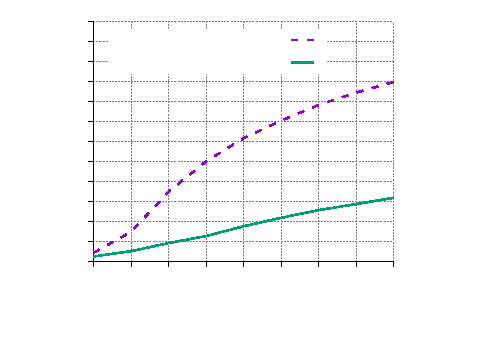
\includegraphics{figures/concat-graph-data.pdf}}%
    \gplfronttext
  \end{picture}%
\endgroup

    \end{subfigure}%
    \hspace{-20pt}
    \begin{subfigure}[t]{0.5\textwidth}
        \centering
        % GNUPLOT: LaTeX picture with Postscript
\begingroup
  \makeatletter
  \providecommand\color[2][]{%
    \GenericError{(gnuplot) \space\space\space\@spaces}{%
      Package color not loaded in conjunction with
      terminal option `colourtext'%
    }{See the gnuplot documentation for explanation.%
    }{Either use 'blacktext' in gnuplot or load the package
      color.sty in LaTeX.}%
    \renewcommand\color[2][]{}%
  }%
  \providecommand\includegraphics[2][]{%
    \GenericError{(gnuplot) \space\space\space\@spaces}{%
      Package graphicx or graphics not loaded%
    }{See the gnuplot documentation for explanation.%
    }{The gnuplot epslatex terminal needs graphicx.sty or graphics.sty.}%
    \renewcommand\includegraphics[2][]{}%
  }%
  \providecommand\rotatebox[2]{#2}%
  \@ifundefined{ifGPcolor}{%
    \newif\ifGPcolor
    \GPcolortrue
  }{}%
  \@ifundefined{ifGPblacktext}{%
    \newif\ifGPblacktext
    \GPblacktexttrue
  }{}%
  % define a \g@addto@macro without @ in the name:
  \let\gplgaddtomacro\g@addto@macro
  % define empty templates for all commands taking text:
  \gdef\gplbacktext{}%
  \gdef\gplfronttext{}%
  \makeatother
  \ifGPblacktext
    % no textcolor at all
    \def\colorrgb#1{}%
    \def\colorgray#1{}%
  \else
    % gray or color?
    \ifGPcolor
      \def\colorrgb#1{\color[rgb]{#1}}%
      \def\colorgray#1{\color[gray]{#1}}%
      \expandafter\def\csname LTw\endcsname{\color{white}}%
      \expandafter\def\csname LTb\endcsname{\color{black}}%
      \expandafter\def\csname LTa\endcsname{\color{black}}%
      \expandafter\def\csname LT0\endcsname{\color[rgb]{1,0,0}}%
      \expandafter\def\csname LT1\endcsname{\color[rgb]{0,1,0}}%
      \expandafter\def\csname LT2\endcsname{\color[rgb]{0,0,1}}%
      \expandafter\def\csname LT3\endcsname{\color[rgb]{1,0,1}}%
      \expandafter\def\csname LT4\endcsname{\color[rgb]{0,1,1}}%
      \expandafter\def\csname LT5\endcsname{\color[rgb]{1,1,0}}%
      \expandafter\def\csname LT6\endcsname{\color[rgb]{0,0,0}}%
      \expandafter\def\csname LT7\endcsname{\color[rgb]{1,0.3,0}}%
      \expandafter\def\csname LT8\endcsname{\color[rgb]{0.5,0.5,0.5}}%
    \else
      % gray
      \def\colorrgb#1{\color{black}}%
      \def\colorgray#1{\color[gray]{#1}}%
      \expandafter\def\csname LTw\endcsname{\color{white}}%
      \expandafter\def\csname LTb\endcsname{\color{black}}%
      \expandafter\def\csname LTa\endcsname{\color{black}}%
      \expandafter\def\csname LT0\endcsname{\color{black}}%
      \expandafter\def\csname LT1\endcsname{\color{black}}%
      \expandafter\def\csname LT2\endcsname{\color{black}}%
      \expandafter\def\csname LT3\endcsname{\color{black}}%
      \expandafter\def\csname LT4\endcsname{\color{black}}%
      \expandafter\def\csname LT5\endcsname{\color{black}}%
      \expandafter\def\csname LT6\endcsname{\color{black}}%
      \expandafter\def\csname LT7\endcsname{\color{black}}%
      \expandafter\def\csname LT8\endcsname{\color{black}}%
    \fi
  \fi
    \setlength{\unitlength}{0.0500bp}%
    \ifx\gptboxheight\undefined%
      \newlength{\gptboxheight}%
      \newlength{\gptboxwidth}%
      \newsavebox{\gptboxtext}%
    \fi%
    \setlength{\fboxrule}{0.5pt}%
    \setlength{\fboxsep}{1pt}%
\begin{picture}(4680.00,3276.00)%
    \gplgaddtomacro\gplbacktext{%
      \csname LTb\endcsname%%
      \put(721,751){\makebox(0,0)[r]{\strut{}$\sfrac{1}{16}$}}%
      \csname LTb\endcsname%%
      \put(721,943){\makebox(0,0)[r]{\strut{}$\sfrac{1}{8}$}}%
      \csname LTb\endcsname%%
      \put(721,1135){\makebox(0,0)[r]{\strut{}$\sfrac{1}{4}$}}%
      \csname LTb\endcsname%%
      \put(721,1327){\makebox(0,0)[r]{\strut{}$\sfrac{1}{2}$}}%
      \csname LTb\endcsname%%
      \put(721,1519){\makebox(0,0)[r]{\strut{}1}}%
      \csname LTb\endcsname%%
      \put(721,1711){\makebox(0,0)[r]{\strut{}2}}%
      \csname LTb\endcsname%%
      \put(721,1903){\makebox(0,0)[r]{\strut{}4}}%
      \csname LTb\endcsname%%
      \put(721,2095){\makebox(0,0)[r]{\strut{}8}}%
      \csname LTb\endcsname%%
      \put(721,2287){\makebox(0,0)[r]{\strut{}16}}%
      \csname LTb\endcsname%%
      \put(721,2479){\makebox(0,0)[r]{\strut{}32}}%
      \csname LTb\endcsname%%
      \put(721,2671){\makebox(0,0)[r]{\strut{}64}}%
      \csname LTb\endcsname%%
      \put(721,2863){\makebox(0,0)[r]{\strut{}128}}%
      \csname LTb\endcsname%%
      \put(721,3055){\makebox(0,0)[r]{\strut{}256}}%
      \csname LTb\endcsname%%
      \put(900,484){\makebox(0,0){\strut{}0}}%
      \csname LTb\endcsname%%
      \put(1260,484){\makebox(0,0){\strut{}}}%
      \csname LTb\endcsname%%
      \put(1620,484){\makebox(0,0){\strut{}100}}%
      \csname LTb\endcsname%%
      \put(1980,484){\makebox(0,0){\strut{}}}%
      \csname LTb\endcsname%%
      \put(2340,484){\makebox(0,0){\strut{}200}}%
      \csname LTb\endcsname%%
      \put(2699,484){\makebox(0,0){\strut{}}}%
      \csname LTb\endcsname%%
      \put(3059,484){\makebox(0,0){\strut{}300}}%
      \csname LTb\endcsname%%
      \put(3419,484){\makebox(0,0){\strut{}}}%
      \csname LTb\endcsname%%
      \put(3779,484){\makebox(0,0){\strut{}400}}%
    }%
    \gplgaddtomacro\gplfronttext{%
      \csname LTb\endcsname%%
      \put(391,1903){\rotatebox{-270}{\makebox(0,0){\strut{}}}}%
      \put(2339,154){\makebox(0,0){\strut{}Number of columns}}%
      \csname LTb\endcsname%%
      \put(3286,1118){\makebox(0,0)[r]{\strut{}implicit join}}%
      \csname LTb\endcsname%%
      \put(3286,898){\makebox(0,0)[r]{\strut{}dependent join}}%
    }%
    \gplbacktext
    \put(0,0){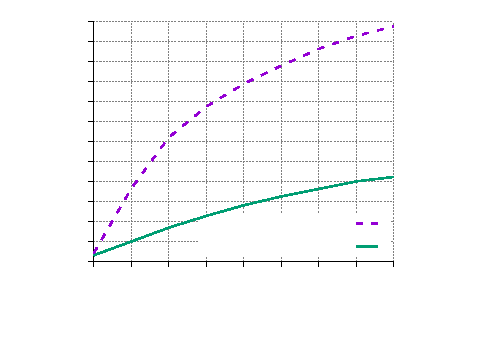
\includegraphics{figures/join-graph-data.pdf}}%
    \gplfronttext
  \end{picture}%
\endgroup

    \end{subfigure}
    \caption{#1}
    \label{fig:dependentVsImplicitBenchmarks}
  \end{figure}
}

\newcommand{\goodreducescalacodesection}{\lstinputlisting[style=scala, firstline=3, lastline=4, breaklines]{scala/src/main/scala/goodreduce.scala}}
\newcommand{\shapecodesection}{\lstinputlisting[style=scala, firstline=8, lastline=11, breaklines]{scala/src/main/scala/numpy.scala}}
\newcommand{\datatypecodesection}{\lstinputlisting[style=scala, firstline=19, lastline=19, breaklines]{scala/src/main/scala/numpy.scala}}
\newcommand{\ndarraycodesection}{\lstinputlisting[style=scala, firstline=23, lastline=23, breaklines]{scala/src/main/scala/numpy.scala}}
\newcommand{\randomnormalcodesection}{\lstinputlisting[style=scala, firstline=27, lastline=27, breaklines]{scala/src/main/scala/numpy.scala}}
\newcommand{\multiplycodesection}{\lstinputlisting[style=scala, firstline=31, lastline=31, breaklines]{scala/src/main/scala/numpy.scala}}
\newcommand{\numelementscodesection}{\lstinputlisting[style=scala, firstline=36, lastline=40, breaklines]{scala/src/main/scala/numpy.scala}}
\newcommand{\reshapecodesection}{\lstinputlisting[style=scala, firstline=44, lastline=45, breaklines]{scala/src/main/scala/numpy.scala}}
\newcommand{\reducecodesection}{\lstinputlisting[style=scala, firstline=50, lastline=66, breaklines]{scala/src/main/scala/numpy.scala}}
\newcommand{\npmeancodesection}{\lstinputlisting[style=scala, firstline=86, lastline=87, breaklines]{scala/src/main/scala/numpy.scala}}
\newcommand{\badreducescalacodesection}{\lstinputlisting[style=scala, firstline=2, lastline=4, breaklines]{scala/src/test/scala/badreduce.scala}}

\hfuzz=0.5pt

%%%%%%%%%%%%%%%%%%%%%%%%%%%%%%%%%%%%%%%%%%%%%%%%%%
%%%%%%%%%%%%%% TypeOf paper headers %%%%%%%%%%%%%%
%%%%%%%%%%%%%%%%%%%%%%%%%%%%%%%%%%%%%%%%%%%%%%%%%%

\newcommand{\oursystem}{$\lambda${\tiny $\mathop{\protect\vphantom{X}}^\text{nd}_{<:\{\}}$}\xspace}
\newcommand\FR{System~FR\xspace}
\newcommand\singleton[1]{\lbrace #1 \rbrace}
\usepackage{xfrac}
\usepackage{caption}
\usepackage{subcaption}
\usepackage{upgreek} % for \textmu

\definecolor{darkblue}{rgb}{0.0, 0.0, 0.55}
\def\diff{\color{darkblue}}
\def\enddiff{}
